\documentclass{article}
\usepackage{amsmath}

\title{Multi-wavefront sensor single-conjugate transfer function derivations}
\author{Aditya R. Sengupta}

\usepackage[margin=0.5in]{geometry}
\usepackage{graphicx}
\usepackage{lipsum}
\usepackage{custom}

\begin{document}
    \maketitle
    \begin{figure}[h]
        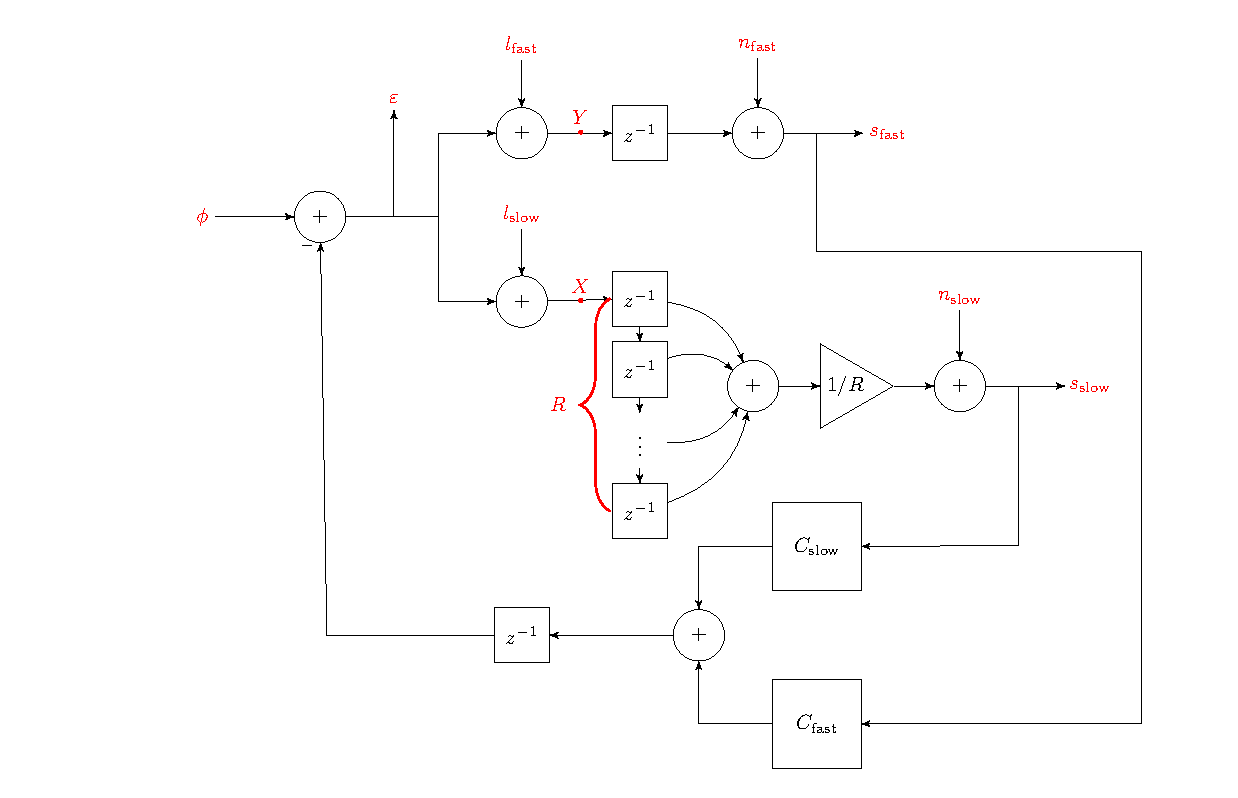
\includegraphics[width=\textwidth]{blockdiag_full.pdf}
    \end{figure}

    We'd like to derive transfer functions between each input ($\phi$, $L_{\text{fast}}$, $L_{\text{slow}}$, $n_{\text{fast}}$, $n_{\text{slow}}$) and output ($X$, the signal seen by the slow WFS; and $Y$, the signal seen by the fast WFS). We do this by writing down relationships between the intermediate named signals, and eliminating any signals other than the input and output.

    Going ``backwards'', we have

    \begin{align*}
        \epsilon &= \phi - D \\
        D &= z^{-1} \parens{C_{\text{fast}} s_{\text{fast}} + C_{\text{slow}} s_{\text{slow}}} \\
        s_{\text{fast}} &= n_{\text{fast}} + z^{-1} Y \\
        Y &= L_{\text{fast}} + \epsilon \\
        s_{\text{slow}} &= n_{\text{slow}} + \frac{1}{R} \parens{\sum_{k=1}^R z^{-k}} X \\
        X &= L_{\text{slow}} + \epsilon \\
    \end{align*}

    To calculate $X/\phi$ and equivalently $Y/\phi$, we set the $L$ and $n$ terms to zero. We're left with $X = Y = \epsilon$.

    \begin{align*}
        X &= \phi - D \\
        D &= z^{-1} \parens{C_{\text{fast}} s_{\text{fast}} + C_{\text{slow}} s_{\text{slow}}} \\
        s_{\text{fast}} &= z^{-1} X \\
        s_{\text{slow}} &= \frac{1}{R} \parens{\sum_{k=1}^R z^{-k}} X \\
    \end{align*}

    This simplifies to

    \begin{align*}
        X &= \phi - z^{-2} C_{\text{fast}} X - z^{-1} C_{\text{slow}} \parens{\sum_{k=1}^R z^{-k}} X\\
        X &\parens{1 + z^{-2} C_{\text{fast}} + z^{-1} C_{\text{slow}} \parens{\sum_{k=1}^R z^{-k}}} = \phi \\ 
        \frac{X}{\phi} &= \frac{1}{1 + z^{-2} C_{\text{fast}} + z^{-1} C_{\text{slow}} \parens{\sum_{k=1}^R z^{-k}}}
    \end{align*}

    For convenience we'll use the name $\text{plant} = z^{-2} C_{\text{fast}} + z^{-1} C_{\text{slow}} \parens{\sum_{k=1}^R z^{-k}}$. This means $X/\phi = Y/\phi = 1 / (1 + \text{plant})$.

    To calculate $X/L_{\text{fast}}$ and $Y/L_{\text{fast}}$, we set $\phi$, $L_{\text{slow}}$, and the $n$ terms to zero.

    \begin{align*}
        X &= -z^{-1} \parens{C_{\text{fast}} z^{-1} Y + C_{\text{slow}} \frac{1}{R} \parens{\sum_{k=1}^R z^{-k}} X} \\
        Y &= L_{\text{fast}} + X \\
    \end{align*}

    We'll first eliminate $Y$ from this:

    \begin{align*}
        X &= -z^{-1} \parens{C_{\text{fast}} z^{-1} \parens{L_{\text{fast}} + X} + C_{\text{slow}} \frac{1}{R} \parens{\sum_{k=1}^R z^{-k}} X} \\
        X & \parens{1 + z^{-2} C_{\text{fast}} X + z^{-1}  C_{\text{slow}} \frac{1}{R} \parens{\sum_{k=1}^R z^{-k}}} = -z^{-2} C_{\text{fast}} L_{\text{fast}}\\
        \frac{X}{L_{\text{fast}}} &= \frac{-z^{-2} C_{\text{fast}}}{1 + z^{-2} C_{\text{fast}} X + z^{-1}  C_{\text{slow}} \frac{1}{R} \parens{\sum_{k=1}^R z^{-k}}} = \frac{-z^{-2} C_{\text{fast}}}{1 + \text{plant}}.
    \end{align*}

    Then, we'll eliminate $X$:

    \begin{align*}
        Y - L_{\text{fast}} &= -z^{-1} \parens{C_{\text{fast}} z^{-1} Y + C_{\text{slow}} \frac{1}{R} \parens{\sum_{k=1}^R z^{-k}} (Y - L_{\text{fast}})} \\
        Y &\parens{1 + z^{-2} C_{\text{fast}} + z^{-1} C_\text{slow} \frac{1}{R} \parens{\sum_{k=1}^R z^{-k}}} = L_{\text{fast}} \parens{1 + z^{-1} C_{\text{slow}} \frac{1}{R} \parens{\sum_{k=1}^R z^{-k}}}\\
        \frac{Y}{L_\text{fast}} &= \frac{1 + z^{-1} C_\text{slow} \frac{1}{R} \parens{\sum_{k=1}^R z^{-k}}}{1 + \text{plant}}.
    \end{align*}

    To calculate $X/L_{\text{slow}}$ and $Y/L_{\text{slow}}$, we set $\phi$, $L_{\text{fast}}$, and the $n$ terms to zero.

    \begin{align*}
        Y &= -z^{-1} \parens{C_{\text{fast}} z^{-1} Y + C_{\text{slow}} \frac{1}{R} \parens{\sum_{k=1}^R z^{-k}} X} \\
        X &= L_{\text{slow}} + Y \\
    \end{align*}

    We'll first eliminate $Y$ from this:

    \begin{align*}
        X - L_{\text{slow}} &= -z^{-1} \parens{C_{\text{fast}} z^{-1} \parens{X - L_{\text{slow}}} + C_{\text{slow}} \frac{1}{R} \parens{\sum_{k=1}^R z^{-k}} X} \\
        X &\parens{1 + z^{-2} C_{\text{fast}} + z^{-1} C_{\text{slow}} \frac{1}{R} \parens{\sum_{k=1}^R z^{-k}}} = L_{\text{slow}} \parens{1 + z^{-2} C_{\text{fast}}}\\
        \frac{X}{L_{\text{slow}}} &= \frac{1 + z^{-2} C_{\text{fast}}}{1 + \text{plant}}.
    \end{align*}

    Then, we'll eliminate $X$:

    \begin{align*}
        Y &= -z^{-1} \parens{C_{\text{fast}} z^{-1} Y + C_{\text{slow}} \frac{1}{R} \parens{\sum_{k=1}^R z^{-k}} (L_{\text{slow}} + Y)} \\
        Y &\parens{1 + z^{-2} C_{\text{fast}} + z^{-1} C_{\text{slow}} \frac{1}{R} \parens{\sum_{k=1}^R z^{-k}}} = L_{\text{slow}} \parens{-z^{-1} C_{\text{slow}} \frac{1}{R} \parens{\sum_{k=1}^R z^{-k}}} \\ 
        \frac{Y}{L_{\text{slow}}} &= \frac{-z^{-1} C_{\text{slow}} \frac{1}{R} \parens{\sum_{k=1}^R z^{-k}}}{1 + \text{plant}}
    \end{align*}

    I'll do the $n$ transfer functions later.
\end{document}